\documentclass[11pt]{article}
\usepackage[T1]{fontenc}
\usepackage[margin=1in]{geometry}
\usepackage{amsmath,amssymb,amsthm}
\usepackage{graphicx}
\usepackage[hidelinks]{hyperref}

\newtheorem*{theorem}{Theorem}
\newtheorem*{lemma}{Lemma}

\newcommand{\R}{\mathbb R}
\newcommand{\E}{\mathbb E}
\newcommand{\sech}{\operatorname{sech}}
\newcommand{\Tr}{\operatorname{Tr}}
\newcommand{\Hess}{\operatorname{Hess}}

\title{A Non-Log-Concave Obstruction to the Marginal Information-Production Inequality}
\author{Run \texttt{fa\_banach\_001}, lane 2}
\date{2026-07-18}

\begin{document}
\maketitle

\section*{Status}

Scoped counterexample, likely valid.  This packet answers the narrow
non-log-concave question around inequality (3.2) in Ball--Nguyen
\cite{BallNguyen2012}.  It does not refute their log-concave entropy-jump
theorem or Lemma 4 under its stated positivity/log-concavity hypothesis.

\section*{Source Question}

The source proves a dimension-free entropy jump for isotropic log-concave
vectors.  Immediately after Theorem 1, it says that log-concavity is crucial
for the proof of inequality (3.2), and that the authors do not know whether
that inequality holds without this assumption.

\begin{center}

\includegraphics[width=0.92\linewidth]{figures/open_question_crop.png}
\end{center}

The inequality in question is the marginal information-production bound from
Lemma 4.  In the notation of the source, if \(h\) is the marginal of a smooth
positive density \(\omega=e^{-\phi}\) under the orthogonal projection onto
\(E\), the displayed bound is
\[
  \int_E \Tr\left[(\Hess \log h)^2\right]h
  \leq
  \int_{\R^N}
  \Tr\left[\left(P_E(\Hess\log\omega)P_E\right)^2\right]\omega .
  \tag{BN}
\]

\begin{center}
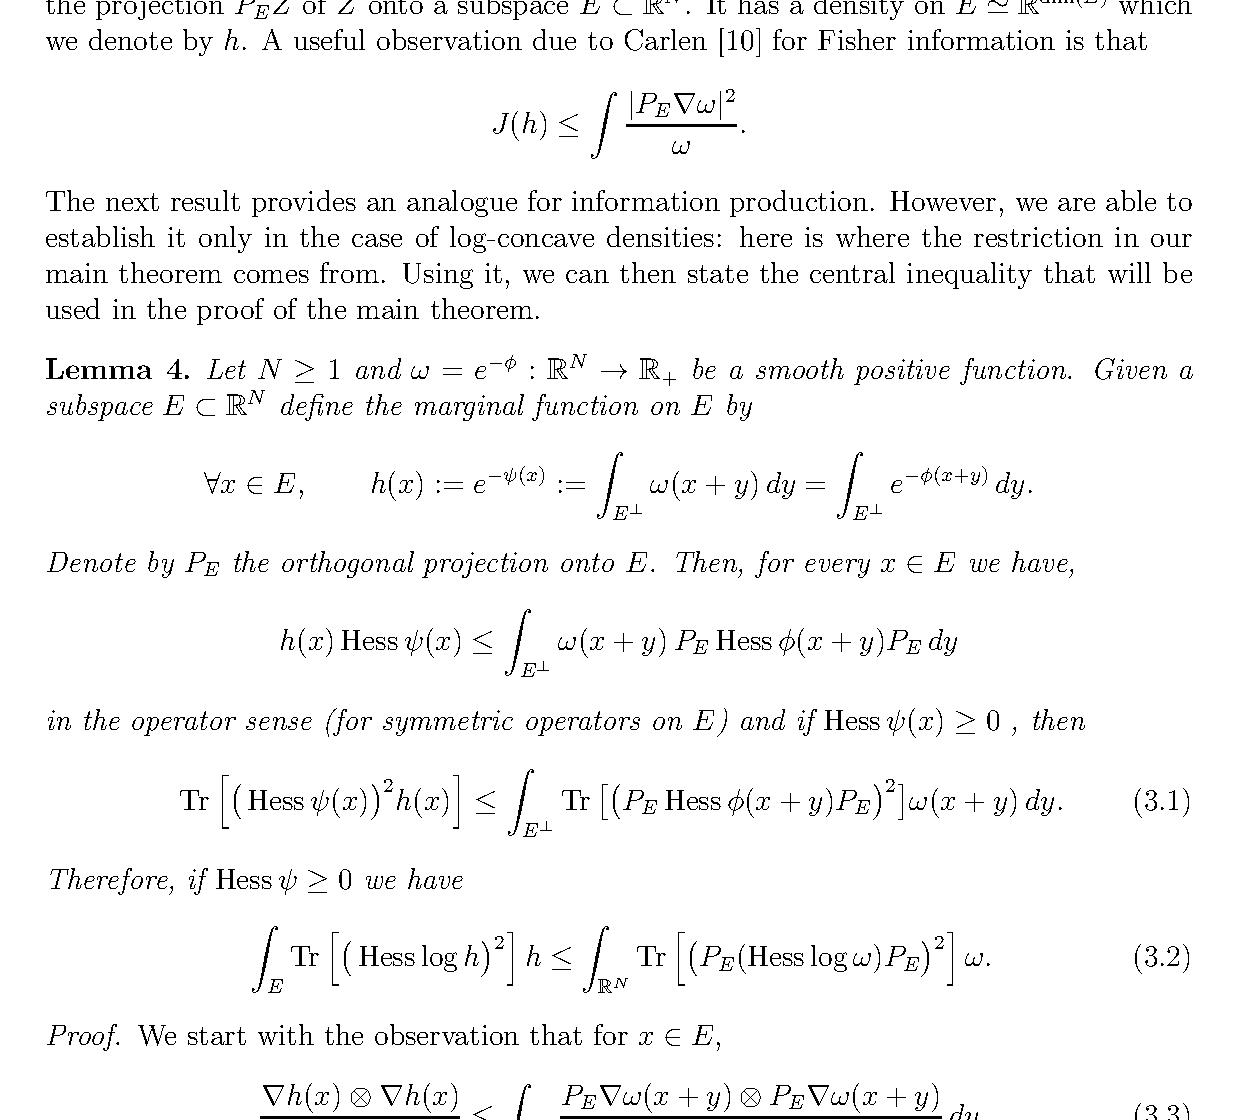
\includegraphics[width=0.92\linewidth]{figures/source_inequality_crop.png}
\end{center}

\section*{Idea of the Proof}

In one dimension, \((\mathrm{BN})\) compares the squared curvature of the log
of a marginal density with the averaged squared \(x\)-curvature of the joint
log-density.  If \(X\mid Y=y\) is always a unit Gaussian with mean depending
on \(y\), then \(\partial_{xx}\log\omega=-1\) everywhere, so the right side is
exactly \(1\).  But if the conditional means are concentrated near two
well-separated values, the \(X\)-marginal is a two-bump Gaussian mixture.
Near the saddle between the two bumps, \(\log h\) has large positive
curvature.  For a suitable separation, the squared curvature integral exceeds
the constant \(1\).

\section*{Counterexample}

\begin{theorem}
The inequality \((\mathrm{BN})\) is false without the log-concavity/sign
mechanism used in Lemma 4 of \cite{BallNguyen2012}.  More precisely, there is
a smooth strictly positive probability density
\(\omega:\R^2\to(0,\infty)\) such that, for the projection
\((x,y)\mapsto x\),
\[
  \int_{\R}\left((\log h)''(x)\right)^2 h(x)\,dx
  >
  \int_{\R^2}\left(\partial_{xx}\log\omega(x,y)\right)^2
  \omega(x,y)\,dx\,dy,
\]
where \(h(x)=\int_{\R}\omega(x,y)\,dy\).
\end{theorem}

\begin{proof}
Let \(a=5/2\).  First consider the limiting one-dimensional mixture
\[
  h_0(x)=\frac12\gamma(x-a)+\frac12\gamma(x+a),
  \qquad
  \gamma(x)=(2\pi)^{-1/2}e^{-x^2/2}.
\]
Equivalently,
\[
  h_0(x)=(2\pi)^{-1/2}e^{-(x^2+a^2)/2}\cosh(ax).
\]
Thus
\[
  (\log h_0)''(x)=-1+a^2\sech^2(ax).
\]
Let
\[
  L_0=\int_\R \left((\log h_0)''(x)\right)^2h_0(x)\,dx .
\]
A direct expansion gives
\[
  L_0-1
  =
  \frac{a^2e^{-a^2/2}}{\sqrt{2\pi}}
  \int_\R e^{-x^2/2}\sech(ax)
  \left(a^2\sech^2(ax)-2\right)\,dx .
  \tag{1}
\]
We show that the integral in (1) is positive for \(a=5/2\).

On \(|x|\leq 0.3\), we have \(a|x|\leq0.75\), hence
\[
  e^{-x^2/2}\sech(ax)\left(a^2\sech^2(ax)-2\right)
  \geq
  e^{-0.045}\sech(0.75)
  \left(\frac{25}{4}\sech^2(0.75)-2\right).
\]
Therefore the contribution of \([-0.3,0.3]\) is larger than
\[
  0.6\,e^{-0.045}\sech(0.75)
  \left(\frac{25}{4}\sech^2(0.75)-2\right)>0.765.
  \tag{2}
\]
The integrand is negative only when
\[
  \sech(ax)<\frac{\sqrt2}{a},
\]
that is, outside
\[
  |x|<\frac{1}{a}\operatorname{arcosh}(a/\sqrt2)>0.46.
\]
On that negative region,
\[
  \left|\sech(ax)(a^2\sech^2(ax)-2)\right|
  \leq 2\sech(ax)\leq 4e^{-a|x|}.
\]
Consequently the total negative contribution is bounded in magnitude by
\[
  8\int_{0.46}^{\infty}e^{-x^2/2-(5/2)x}\,dx
  =
  8e^{25/8}\sqrt{\frac{\pi}{2}}\,
  \operatorname{erfc}\!\left(\frac{2.96}{\sqrt2}\right)
  <0.703 .
  \tag{3}
\]
The lower bound (2) and upper bound (3) prove that the integral in (1) is
positive.  Hence \(L_0>1\).

Now smooth the two-point mixer.  Let \(Y_\sigma\) have density
\[
  p_\sigma(y)=\frac12\frac{1}{\sigma}\gamma\!\left(\frac{y-1}{\sigma}\right)
  +\frac12\frac{1}{\sigma}\gamma\!\left(\frac{y+1}{\sigma}\right),
\]
and, conditionally on \(Y_\sigma=y\), let \(X_\sigma\) be Gaussian with mean
\(ay\) and variance \(1\).  The joint density is
\[
  \omega_\sigma(x,y)=p_\sigma(y)\gamma(x-ay),
\]
which is smooth and strictly positive on \(\R^2\).  Since
\[
  \partial_{xx}\log\omega_\sigma(x,y)=-1
\]
everywhere, the right side of \((\mathrm{BN})\) for the projection onto the
\(x\)-axis is exactly
\[
  \int_{\R^2}1\cdot\omega_\sigma(x,y)\,dx\,dy=1.
\]

The \(x\)-marginal of \(\omega_\sigma\) is
\[
  h_\sigma(x)=
  \frac12\gamma_s(x-a)+\frac12\gamma_s(x+a),
  \qquad
  s^2=1+a^2\sigma^2,
\]
where \(\gamma_s\) is the centered Gaussian density of variance \(s^2\).  As
\(\sigma\downarrow0\), \(h_\sigma\) and the first two derivatives of
\(\log h_\sigma\) converge pointwise to the corresponding quantities for
\(h_0\); on \(0\leq\sigma\leq\sigma_0\) they are dominated by an integrable
Gaussian-tail bound.  Dominated convergence gives
\[
  \int_\R \left((\log h_\sigma)''(x)\right)^2h_\sigma(x)\,dx
  \longrightarrow L_0>1.
\]
Thus, for all sufficiently small positive \(\sigma\), the left side of
\((\mathrm{BN})\) is larger than \(1\), while the right side is exactly \(1\).
This proves the claimed smooth positive-density counterexample.
\end{proof}

\section*{Verification Notes}

The proof above is analytic.  The script
\texttt{code/mixture\_curvature\_check.py} only checks the numerical size of
the gap for finite smoothing.  For \(a=5/2\), it prints values such as
\[
  L_{0.05}-1 \approx 0.143185>0.
\]
This supports the continuity step but is not used as a proof.

\section*{Limitations}

This packet refutes only the log-concavity-free version of \((\mathrm{BN})\).
It leaves intact:
\begin{itemize}
\item the source theorem for isotropic log-concave random vectors;
\item Lemma 4 under the stated \(\Hess\psi\geq0\) sign condition;
\item any non-log-concave variant that imposes a replacement sign condition on
the marginal potential \(\psi=-\log h\).
\end{itemize}

\section*{Novelty and Search Bounds}

Local cheap indexes were searched for arXiv:1206.5098, entropy jumps,
information production, log-concavity, marginal Hessian inequalities, KLS,
thin shell, and slicing/hyperplane.  Existing run memory already covers the
later resolution of slicing/hyperplane and thin-shell conjecture targets, but
no packet covered this non-log-concave marginal-information inequality.

Web searches on 2026-07-18 for the source title, the phrase ``we do not know
whether'', ``marg1bis'', ``information production marginal log-concave'', and
nearby entropy-jump literature found the source paper and later log-concave
extensions such as Bizeul \cite{Bizeul2023}, but no explicit counterexample to
the non-log-concave form of \((\mathrm{BN})\).

\section*{Human Review Recommendation}

Accept as a scoped counterexample to removing log-concavity/sign assumptions
from the marginal information-production inequality (3.2).  Do not count it as
a counterexample to the source's log-concave entropy-jump theorem.

\begin{thebibliography}{9}

\bibitem{BallNguyen2012}
K. Ball and V. H. Nguyen,
\emph{Entropy jumps for isotropic log-concave random vectors and spectral gap},
Studia Math. 213 (2012), no. 1, 81--96.  arXiv:1206.5098.

\bibitem{Bizeul2023}
P. Bizeul,
\emph{Entropy and Information jump for log-concave vectors},
Comptes Rendus. Mathematique 361 (2023), 487--493.

\end{thebibliography}

\end{document}
